\documentclass[12pt]{article}
\usepackage{setspace}
\usepackage[margin = 1.4in]{geometry}
\usepackage{amsfonts, amsmath, amssymb}
\usepackage[none]{hyphenat}
\usepackage{graphicx}

\begin{document}
\begin{titlepage}
   \vspace*{\stretch{1.0}}
   \begin{center}
      \Large\textbf{Genetic Alogrithm for CNN Hyperparametr Optimization}\\
      \vspace*{\stretch{0.3}}
      \large\textit{Tianrui Guo}\\
      \vspace*{\stretch{0.1}}
      \large Department of Applied Mathematics\\
      \vspace*{\stretch{0.1}}
      \large\textit{April 20, 2019}
   \end{center}
   \vspace*{\stretch{2.0}}
\end{titlepage}

\pagebreak
\setlength{\baselineskip}{10mm}
\begin{center}
\LARGE \textbf{Abstract}
\end{center}
In this big data era, we developed many efficient and effective ways to analyze our database. Among various techniques, computer vision is a fancy and important one. One of the most significant technique in modern computer vision is convolutional neural network which is a typical method in deep learning. When we process image classification or image recognition, we inevitably encounter a problem of determine the hyperparamters such as the number of Conv channels, the size of filters or the dimension of the dense layers. The process of finding a set of hyperparameters which can improve the performance of convolutional neural network is known as hyperparameter optimization, and it can be also called as tuning. In this Capstone project we are using genetic algorithm for finding an optimal CNN architecture. When the convolutional neural network goes deeper and more complicated, the number of hyperparameters increases dramatically. In order to increase the performance of tuning, we no longer use manual tuning methods like grid search,  instead we use genetic algorithm which is a kind of random search method for tuning, because we want the optimization algorithm searching automatically in a larger hyperparamter space.  To test the performance of genetic tuning, we implement genetic algorithm on MNIST which is a relative small data set include 60,000 examples in training set and 10,000 examples in test set. If this algorithm performs well in this dataset, we will have possibility to implement it on other significative datasets.\pagebreak
\section{Introduction}
Machine learning is the cutting edge technique in modern data science, and it is dominated by deep neural network. These great inventions enable us have much better performance in data analysis. Inspired by the deep neural network architecture, we obtain a rapid development in computer vision. Computer vision is an cutting edge technique making computer to see visual object and extract information from images and videos in the similar way as human does. Image classification and image recognition are the art-of-state field in computer vision, and they have significant contribution to human face recognition, automatic driving and neural style transfer. In this capstone project, we are using convolutional neural network to train MNIST dataset, and this is a kind of image classification. MNIST dataset is a large database of handwritten digits that is commonly used for training various image processing systems. The examples in MNIST dataset are black and white images of human handwritten digits and they are normalized to fit into a $28 \times 28$ pixel bounding box and anti-aliased, which introduced grayscale levels. Hence, we can encode the images into matrices which have all entries equals to one or zero, this problem is transferred as matrix regression. The framework we use to process image classification of MNIST dataset is convolutional neural network (we called CNN or Conv neural network later). Convolutional neural network (CNN, or ConvNet) is a class of deep neural networks, most commonly applied to analyzing visual imagery. Convolutional networks were inspired by biological mechanism in that the connectivity pattern between neurons resembles the organization of the animal visual cortex. The advantage of CNN of image classification is CNN has a weight-sharing feature. Comparing with fully connected neural networks, CNN has conspicuous fewer parameters which makes CNN extract information from dataset at lower computational cost. \\
~\\
The main purpose of this project is to find an optimal hyperparameter set for CNN framework. In deep learning, a hyperparameter is a parameter whose value is set before the training begins. Different models have different types of hyperparameters, in our CNN model we have filter size, Conv layer channel, pooling size, drop out rate and dense layer size as hyperparameters. Hyperparameters are integers and continuous numbers in our model, leading to mixed-type optimization problems. The choice of hyperparameters can affect the performance of deep neural network significantly. The accuracy and the time required for training process will depend on the hyperparameters we choose. To improve performance of our CNN model, we can apply various tuning methods to find a set of optimal hyperparameters. In this case we are applying genetic algorithm for hyperparameter optimization. Genetic algorithm for CNN tuning is a kind of population based training which is inspired by the process of natural selection. We consider a tuple of hyperparameters as a chromosome of an individual. In our model, we assume every individual has only one chromosome. Since one chromosome represents a tuple of hyperparameters, a gene on the chromosome represents one hyperparameter. If a model has ten hyperparameter, the individual will have one chromosome consists ten genes. For our genetic algorithm, all the individuals in the same generation constitute the whole population. In next section, we will discuss each gene on the chromosome and how genetic algorithm works. For the first generation, we randomize the initial population using the hyperparameter distribution that is pre-defined. In this case, we regulate the distribution of hyperparameter to save computational resource, since genetic algorithm is at high level of computational cost, and we will also discuss later. Compare to using grid search method, for the first generation, we use random method to generate will enable us to explore more combination of hyperparameters. In most cases, we know little about the properties of deep neural ntework model, so that it is hard to directly give empirical combinations which have great performance. Even though grid search method seems more robust, we will not use it here. Figure \ref{fig:pic1} shows difference between grid search and random search.\\
~\\
The remainder of this Capstone project is organized as follows. In Section 2 we will discuss the model and tuning method we use. Section 2.1 is about CNN model for this problem, and Section 2.2 is about genetic algorithm.  Results after testing by MNIST dataset are included in Section 3 and we draw conclusion in Section 4.  \\
\begin{figure}\label{fig:pic1}
\begin{center}
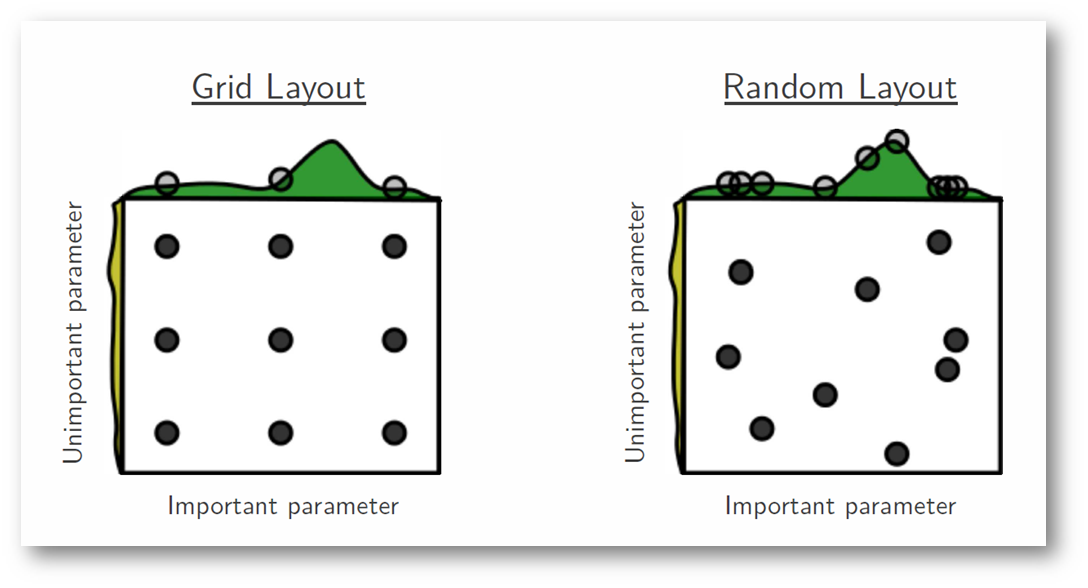
\includegraphics[width = 5.5in]{grid_vs_random.png}
\caption{Grid Search vs Random Search}
\end{center}
\end{figure}
%\begin{align}\label{eqn:22}
%x=2s
%\end{align}
%IN \eqref{eqn:22}, we consider the interaction 



\section{Modeling}
In the first part of this section, we will discuss the structure of our CNN model, and explain the functions of every part of CNN architecture. In the second part of this section we will introduce genetic algorithm, and we will explain how genetic algorithm works for CNN hyperparameter tuning. In our model for training MNIST dataset, CNN model is implemented as the inner part for genetic algorithm, and genetic algorithm works as outer structure for selecting optimal hyperparameter combination.
\begin{figure}\label{fig:pic2}
\begin{center}
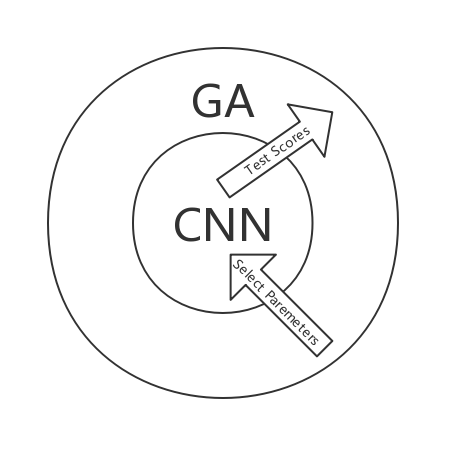
\includegraphics[width = 3.2in]{relationships.png}
\caption{Relationship bewteen genetic algorithm and CNN in our model}
\end{center}
\end{figure}
\subsection{CNN Model}
As the inner structure of our model, CNN model is the classifier that test the performance of the model by a tuple of given hyperparameters from genetic algorithm. In our experiment, we use fixed layer structure to train MNIST dataset. In other words, our neural layers such as Conv layers, max pooling layers, drop-out layers, dense layers and softmax layers are in fixed order and the number of each layer is also fixed. The reason that we are not using a dynamic structure CNN model is because we are tuning the model by genetic algorithm, therefore the individual in a certain generation will have the same type of chromosome which indicate they have the same type of genes representing hyperparameters. If we change the order or number of our hidden layers in CNN model, the chromosome of individuals will change simultaneously. Individual with different type of chromosome cannot reproduce the next generation.\\
~\\
The structure that we are applying is shown in Figure 3. 
\begin{figure}\label{fig:pic3}
\begin{center}
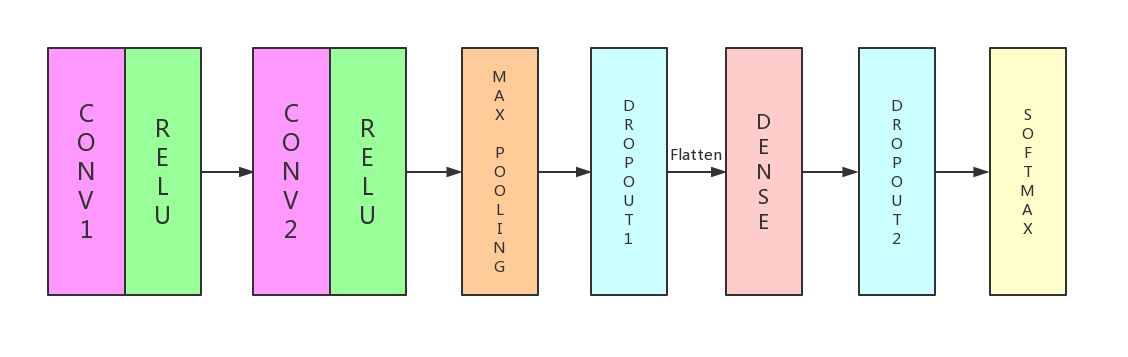
\includegraphics[width = 6.1in]{CNN.png}
\caption{The structure of our CNN model}
\end{center}
\end{figure}
This model is inspired by LeNet-5, which is developed by Yann Lecun. The first hidden unit is consisted of a convolution operator and a ReLU activation function. The convolution operator calculates the summation of the production between each entry in the filter matrix and the corresponding area in the input matrix. Here we applied $1$ as the strides of filter since our input is just a $28 \times 28$ gray scale image, we do not use bigger strides. Consider $A$ is the input matrix, $A_R $ is the sub-matrix of $A$ whose upper left entry is $A_{ij}$ and dimension equals to $m$ which is the dimension of filter maxtix and $F$ is the filter matrix. Then we have:\\
$$Conv(A)_{ij} = \displaystyle\sum_{p=1}^{m}  \displaystyle\sum_{q=1}^{m} {A_R}_{pq}F_{pq}$$Figure 4 shows how the convolution operator works. In this case, the first hidden layer provides us two hyperparameters which are the size of filter(or kernel) and the number of filters. It worth to notice that we actually apply same padding to the input matrix. For MNIST dataset, the inputs of data $28 \times 28$ pixel image, this is of a very small dimension. We basically don not want the image shrink when processing Conv layers, so we just add zero entries around the input matrix to get the output matrix ad the same dimension after Conv layers, and this is what we do for same padding. Additionally, if we do not  use any padding, the entries near the boundaries of input matrix will become less import.\\
\begin{figure}
\begin{center}
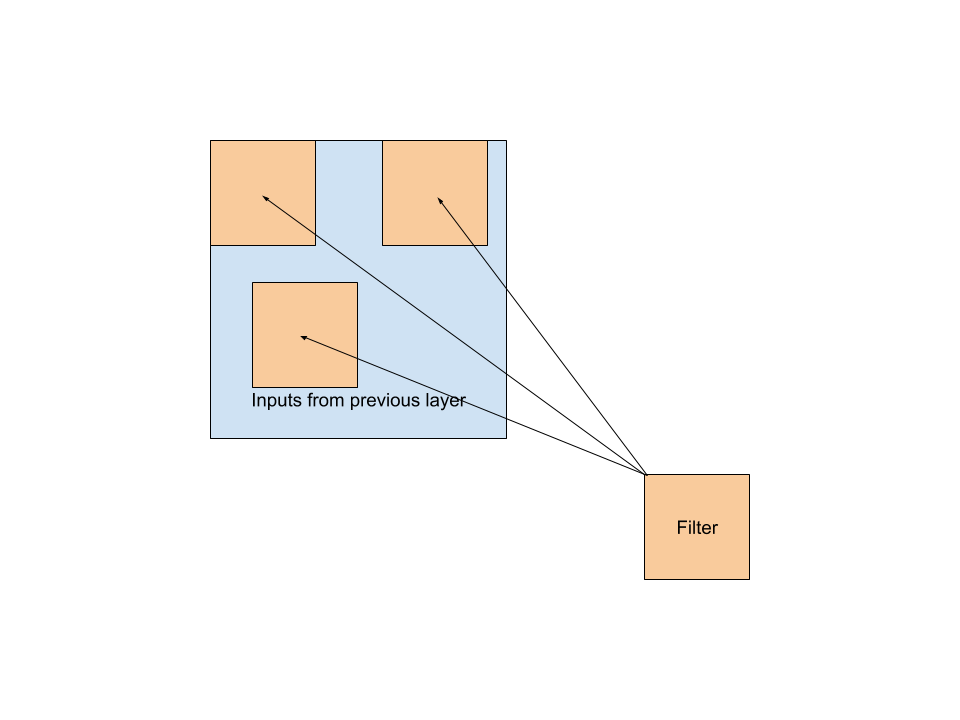
\includegraphics[width =4.7in]{filter.png}
\caption{How CNN filter and max pooling layer works}
\end{center}
\label{fig:pic4}
\end{figure}
~\\
After the convolution operation, we put the matrix into an activation function. In our cases, we use ReLU. This activation function was first introduced to a dynamical network by Hahnloser et al. in 2000. The mathematical notation of ReLU is:
$$f(x) = max(0, x) = x^+$$
ReLU function helps us map the output of previous layer to the range of 0 to 1. The reason that we use ReLU as activation function is:
\begin{itemize}
  \item \textbf{Sparsity}: When the input of ReLU is non-positive, the output turns to be zero, which sparse activation.
  \item \textbf{Better gradient propagation}: ReLU can effectively reduce vanishing gradient problem. For example, the gradient of sigmoid activate function vanishes when the absolute value of input goes very large.
  \item \textbf{Easy to compute}: ReLU save a lot of computational resource when doing propagation.
 \end{itemize}
For the second hidden unit, it is totally the same with the first one, and also gives us another two hyperparameters which are the size of the filers and the number of filters. This hidden unit is following with a max pooling layer. The max pooling layer works similarly as Conv layers, the Conv layers calculate the summation of the productions of each pair of entries in input matrix and filter matrix. The max pooling layer just selects the max entry of each sub-matrix in the same size as the max pooling kernel. In Figure 4, max pooling layer just select the max values in those yellow boxes. The purpose that we add pooling layers in our neural network is the pooling layers can reduce the size of the representations and keep the significant values which accelerate our computation. Notice that the max pooling layer also provide us a new hyperparameter which is the size of max pooling kernel. The next layer of our model is a dropout layer. This layer works in a quite simple way but it will help our model get better convergence. The dropout layer randomly drop some hidden units in our neural network, in other words, we ignore some neurons in forward or backward propagation. By doing this we can effectively prevent over-fitting, and this dropout layer gives us a hyperparameter of the random drop rate. Until this part, we finished the feature learning of our model, and the next thing we need to do is the classification part, which enable us to get the relationship between images and labels. Firstly we need to apply a fully connected layer to the output from previous convolutional layers. Before doing this, we need to flatten the output matrices from Conv layers. This means we reshape tensor into vector in order to proceed the fully connected layer. A fully connected layer is an linear operation in which each input is connected to each output by a weight and a bias. Suppose $a^{[l-1]}$ is the  input vector of the $l-1^{th}$ layer, $W^{[l]}_i$ is the $i^{th}$ weight vector in the next $l^{th}$ layer, and $b_i$ is the $i^{th}$ bias, then we will have $a^{[l]}_i$ which is the $i^{th}$ output of $l^{th}$ dense layer(fully connected layer is also called dense layer) is:
$$a^{[l]}_i = ReLU(W^{[l]}_i a^{[l-1]} + b_i)$$
$ReLU$ is the activation function we use before. This dense layer also provides a hyperparameter of the output vector size. This means the number of the weight vector multiplied by the flattened input vector. The first fully connected layer is also followed by a dropout layer that deactivate some neurons to improve the convergence a prevent over-fitting which gives us a dropout rate as another hyperparameter. \\
~\\
The final layer of CNN model is also a dense layer, but different from the previous dense layer, we are applying another activation function which is Softmax Function. The reason that we use Softmax function is because we are doing multiple classification. MNIST dataset has ten categories of labels for human-written images, so the out put of our CNN model should give us corresponding outputs. The activation function such as ReLU and sigmoid can only do binary classification, and that is why we cannot use them in the final layer to generate outputs. Suppose $z^{[l]}_i$ is the value after linear operation $W^{[l]}_i a^{[l-1]} + b_i$ for the $l^{th}$ dense layer. The mathematical equation of Softmax function is:
$$Softmax(z^{[l]}_i) = \frac{e^{z^{[l]}_i}}{\displaystyle \sum_{i=1}^me^{z^{[l]}_i}}$$
where $m$ is the number of categories, in our case $m=10$. The Softmax activation function gives us output of multiple catrgories. From the equation above, we will get an output of probabilities of each label, and then the Softmax layer return us a corresponding label. For instance, in the MNIST problem, if the probability of number $1$ is the maximum value among all probabilities it will return the label as $1$. By using Softmax function, we got the final output of forward propagation. \\
~\\
For deep neural network, the choice of loss function and optimizer can significantly affect the performance of the model. When we use Softmax as activation function, the categorical Cross-Entropy loss can be a good choice for
our regression. The reason we choose categorical Cross-Entropy loss is we are doing a multi-class classification, and categorical Cross-Entropy loss cooperates with Softmax very well. The formula of categorical Cross-Entropy loss in our case is:
$$CELoss = -\displaystyle\sum_i^ct_ilog(Softmax(s)_i)$$
$$t_{i=p} = 1, t_{i \neq p} = 0$$
In this formula, $c$ is the number of classes(labels), $t$ is a $c$ dimension vector of $0s$ and $1s$. For the output is  one-hot, only when the $p^{th}$ class keeps its term, the $p^{th}$ entry of $t$ equals to $1$, otherwise the entries of $t$ is zero and $s$ is the output of CNN model. In our case, the output is a vector with probabilities so the formula can be written as:
$$CELoss = -\displaystyle\sum_i^n \hat{y_{i1}}log(y_{i1})+\hat{y_{i2}}log(y_{i2})+\cdots+\hat{y_{ic}}log(y_{ic})$$
where $n$ is the number of samples and $c$ is the number of categories. The optimizer we apply is ADADELTA method. We actually do not tuning our learning rate, therefore we use ADADELTA since it has a robust performance even if using the default learning rate in most cases. It is also worth to mention that we are using mini batch gradient descent method for training, this will help us get a better and faster convergence. Hence we get another hyperparameter of batch size.\\
~\\
Until now, our model basically needs to optimize nine hyperparameters, they are:
\begin{itemize}
\item The size of filters for the first and second Conv layers
\item The number of filters for the first and second Conv layers
\item The dropout rates for the two dropout layers
\item The dimension for the two dense layers
\item The mini batch size
\end{itemize}
Notice that we do not take the number of epoch as a hyperparameter because there will be a great difference between different epoch, this hyperparameter will vanish the influence of other hyperparameter. In the second part, we will discuss how does genetic algorithm work with hyperparameter optimization.



\subsection{Genetic Algorithm}
There are many advantages of using genetic algorithm for hyperparameter optimization:
\section{Result}

\section{Conclusion}

\end{document}